\chapter{Deepfake methods}
\section{Autoencoder}
\label{Autoencoder}
Autoencoders are the most basic approach to the problem of deepfake generation. In fact, all mentioned methods, except for CycleGAN, are just different variations of this idea. Autoencoder is a type of artificial neural network that learns to reproduce given input in an unsupervised manner. The goal is to train functions \(A: \mathbb{R}^n \to \mathbb{R}^p\) (encoder) and \(B: \mathbb{R}^p \to \mathbb{R}^n\) (decoder) to satisfy condition given in equation \ref{eq:autoencoder_condition} as described in \cite{autoencoders_bib},
%
\begin{equation}
\label{eq:autoencoder_condition}
arg \, min_{A,B} E[\Delta(x,B \circ A(x))]
\end{equation}
%
where \(E\) -- expectation over the distribution of \(x\) and \(\Delta\) -- reconstruction loss function, which measures the distance between given input and the output of the decoder. General idea of autoencoder model is illustrated in figure \ref{fig:autoencoder_general_idea}. Typically, architecture of autoencoder consists not only of input and output layers, as this would result in simple coping pixels from the input to the output of the network, but also contains single or multiple hidden layers in between, with the number of neurons lesser than the number of pixels in the input image. Such structure causes bottleneck effect and creates so-called compressed representation at the output of the encoder part, known also as ``feature map'' or in case of deepfake ``latent face''. Such compression causes feature map to preserve only information most relevant for later reconstruction and gets rid of unnecessary data.

\begin{figure}[H]
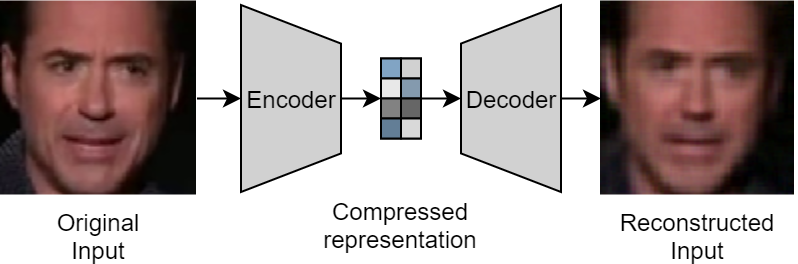
\includegraphics[width=12cm] {autoencoder_general_idea.png}
\centering
\caption{General idea of autoencoder}
\label{fig:autoencoder_general_idea}
\end{figure}

Generating deepfakes using autoencoders approach consists of three major steps. Described process is illustrated in figure \ref{fig:deepfake_steps}. Let us assume that \(X\) is a set of face images of person \(x\) and \(Y\) is a set of face images of person \(y\). Firstly, as shown in figure \ref{subfig:deepfake_steps_a}, an encoder is trained to produce feature maps for images of faces from both classes. Simultaneously, a corresponding decoder (further called decoder XY) is trained as a measure of encoder accuracy. Afterwards, two decoders (further called decoder X and decoder Y) are trained separately to reproduce original images from latent faces generated by pre-trained encoder, as presented in figure \ref{subfig:deepfake_steps_b}. Finally, decoders are switched to produce images from one class based on feature maps from the other class, which was illustrated in figure \ref{subfig:deepfake_steps_c}.

\begin{figure}[H]
\centering
\begin{subfigure}{12cm}
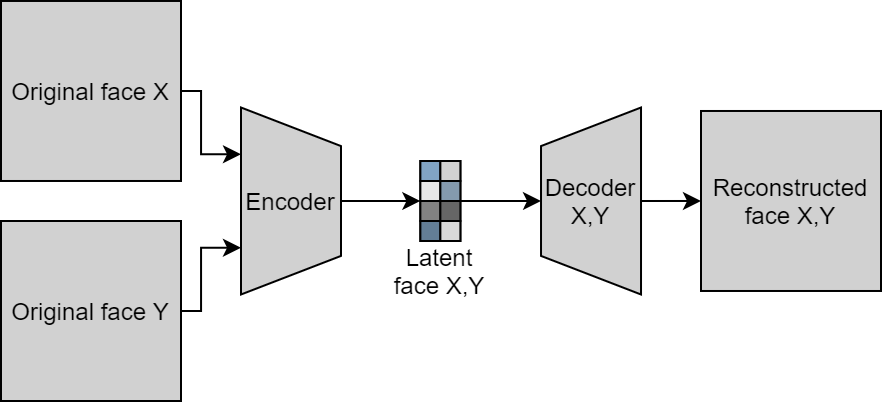
\includegraphics[width=\textwidth]{deepfake_idea_1.png}
\caption{Training autoencoder}
\label{subfig:deepfake_steps_a}
\end{subfigure}

\begin{subfigure}{12cm}
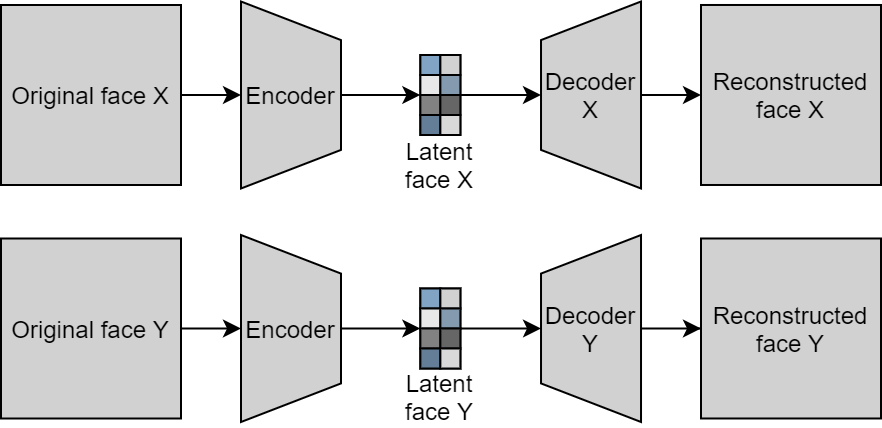
\includegraphics[width=\textwidth]{deepfake_idea_2.png}
\caption{Training decoders X and Y}
\label{subfig:deepfake_steps_b}
\end{subfigure}

\begin{subfigure}{12cm}
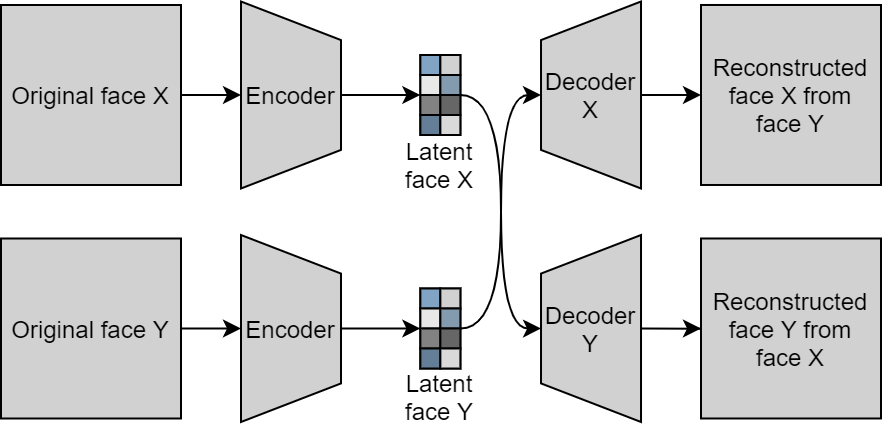
\includegraphics[width=\textwidth]{deepfake_idea_3.png}
\caption{Generating X from Y and Y from X}
\label{subfig:deepfake_steps_c}
\end{subfigure}

\caption{Three steps of generating deepfakes}
\label{fig:deepfake_steps}
\end{figure}

\newpage
\section{Variational autoencoder}
\label{Variational_autoencoder}
Unlike basic autoencoders, which purpose is to reproduce given input by ``memorizing'' it, variational autoencoders aim to produce latent vectors (feature maps) that follow a unit Gaussian distribution \cite{variational_bayes_bib}. Such modification allows to generate new images by sampling a latent vector from the unit Gaussian distribution and pass it as an input of the decoder network. The goal in VAE model training is to optimize the loss function given in equation \ref{eq:vae_loss} \cite{vae_loss_bib}. First component of this function is a reconstruction loss \(\mathcal{L}_{rec}\), which, by comparing pixels from image \(x\), encoded to a latent vector \(z = Encoder(x) \sim q(z|x)\), and reconstructed image \(\bar{x} = Decoder(z) \sim p(x|z)\), measures expected marginal log-likelihood of the observations in \(x\). Second component, so called Kullback–Leibler divergence \cite{kl_divergence_bib}, measures the extent to which one probability distribution differs from another. Applying KL divergence to VAE loss function allows to control distribution of the latent vector \(z\).
%
\begin{equation}
\label{eq:vae_loss}
\mathcal{L}_{vae} = \mathcal{L}_{rec} + \mathcal{L}_{kl}
\end{equation}
%
\begin{equation}
\label{eq:rec_loss}
\mathcal{L}_{rec} = -E_{q(z|x)}[\log{p(x|z)}]
\end{equation}
%
\begin{equation}
\label{eq:kl_loss}
\mathcal{L}_{kl} = D_{kl}(q(z|x)||p(z|x))
\end{equation}

Presence of KL divergence in VAE loss function generates problem with applying backpropagation to the encoder network, as decoder randomly samples from latent vector \(z\) and backpropagation cannot flow through random node as in figure \ref{subfig:before_reparameterization}. As a solution, a ``reparameterization trick'' is introduced \cite{reparameterization_trick_bib}. This method maps the output of an encoder to separate vectors, mean \(\mu\) and standard deviation \(\sigma\), instead of a z-dimensional latent vector. Such representation allows to calculate \(z\) in a following way:
%
\begin{equation}
\label{eq:rec_loss}
z = \mu + \sigma\epsilon
\end{equation}
%
where \(\epsilon\) is sampled from a multivariate standard normal distribution (\(Normal(0,1)\)) and therefore acts as a stochastic component. Such reparameterization allows to run backpropagation process as now latent vector is not purely random, but consists of deterministic and stochastic nodes as illustrated in figure \ref{subfig:after_reparameterization}.

\begin{figure}[H]
\centering
\begin{subfigure}{.5\textwidth}
  \centering
  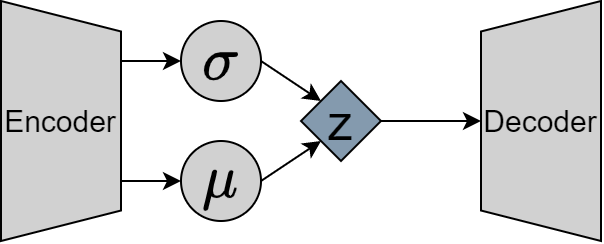
\includegraphics[width=0.9\linewidth]{before_reparameterization.png}
  \caption{Nodes before reparameterization}
  \label{subfig:before_reparameterization}
\end{subfigure}%
\begin{subfigure}{.5\textwidth}
  \centering
  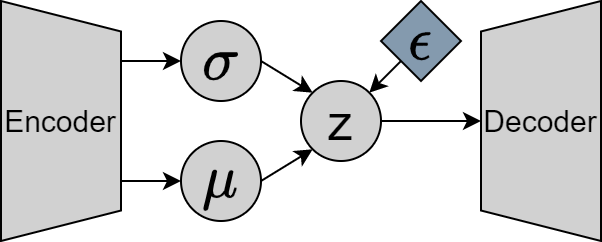
\includegraphics[width=0.9\linewidth]{after_reparameterization.png}
  \caption{Nodes after reparameterization}
  \label{subfig:after_reparameterization}
\end{subfigure}
\caption{Reparameterization trick}
\label{fig:reparameterization_trick}
\end{figure}

By applying reparameterization trick to equation \ref{eq:kl_loss}, Kullback–Leibler divergence takes following form \cite{kl_divergence_loss_bib}:
%
\begin{equation}
\label{eq:final_kl_loss}
\mathcal{L}_{kl} = -\frac{1}{2}\sum_{i=0}^{z}(1 + \log(\sigma_i^2) - \mu_i^2 -\sigma_i^2)
\end{equation}

Generating deepfakes using variational autoencoders approach is based on the same algorithm as autoencoders approach illustrated in figure \ref{fig:deepfake_steps}. The only difference between those two methods is the way the latent face (latent vector) is obtained.

\section{VAE-GAN}
\label{VAE-GAN}
As the name suggests, variational autoencoder generative adversarial network is a combination of previously mentioned VAEs and GANs. By combining those two approaches it is possible to leverage learned representations to better measure similarities in data space \cite{autoencoding_beyond_pixels_bib}. General idea of this technique is similar to the one described in section \ref{Variational_autoencoder}, but instead of VAE's decoder, a GAN generator is used to decode feature maps, as illustrated in figure \ref{fig:vaegan_general_idea}.

\begin{figure}[H]
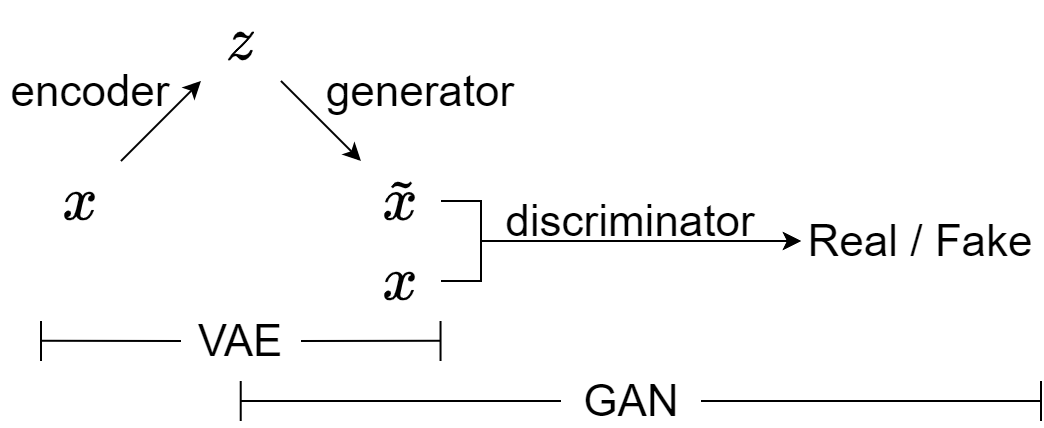
\includegraphics[width=9cm] {vaegan_general_idea.png}
\centering
\caption{General idea of VAE-GAN}
\label{fig:vaegan_general_idea}
\end{figure}

The whole potential of this method comes from the discriminator part. This network, during the training process, learns to distinguish real images (pictures before encoding) from generated ones. On the other side, generator network ``tries'' to deceive the discriminator by producing better and better fake images, improving the quality of final deepfakes. General idea of GAN training process is illustrated in figure \ref{fig:gan_general_idea}. To train VAE-GAN model, three different loss functions, applied to corresponding networks, are required: encoder loss, generator loss and discriminator loss:
%
\begin{equation}
\label{eq:encoder_loss}
\mathcal{L}_{Enc} = -E_{q(z|x)}[\log{p(x|z)}] + D_{kl}(q(z|x)||p(z|x))
\end{equation}
%
\begin{equation}
\label{eq:generator_loss}
\mathcal{L}_{Gen} = -E_{q(z|x)}[\log{p(x|z)}] * \gamma - \log(Dis(X)) - \log(1 - Dis(\tilde{X}))
\end{equation}
%
\begin{equation}
\label{eq:discriminator_loss}
\mathcal{L}_{Dis} = \log(Dis(X)) + \log(1 - Dis(\tilde{X}))
\end{equation}
%
where \(\tilde{X}\) - fake image generated from encoded image \(X\), \(\gamma\) - weight factor to balance the loss function value. 

\begin{figure}[H]
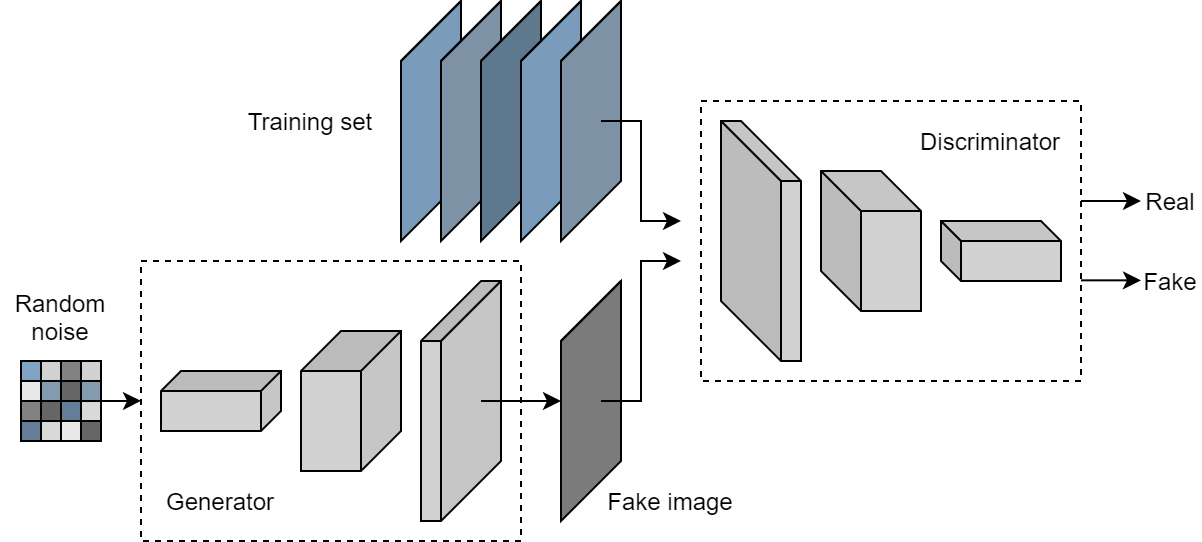
\includegraphics[width=14cm] {gan_general_idea.png}
\centering
\caption{General idea of GAN}
\label{fig:gan_general_idea}
\end{figure}

\section{CycleGAN}
CycleGAN is an approach to the image-to-image translation problems, based on deep learning techniques, which does not require a dataset of paired images. Typically, CycleGAN model's architecture consists of two GAN networks, where one generator (\(G:X \to Y\)) is responsible for generating images for one class, and the other (\(F:Y \to X\)) for generating images for the second one \cite{cycleGAN_4_bib}. The goal of the training process is given in the equation \ref{eq:cyclegan_condition1}, as described in \cite{cycleGAN_5_bib},
%
\begin{equation}
\label{eq:cyclegan_condition1}
G^*,F^* = arg \, \min_{G,F} \, \max_{D_X,D_Y} \mathcal{L}(G,F,D_X,D_Y)
\end{equation}
%
\begin{equation}
\label{eq:cyclegan_condition2}
\mathcal{L}(G,F,D_X,D_Y) = \mathcal{L}_{GAN}(G,D_Y,X,Y) + \mathcal{L}_{GAN}(F,D_X,Y,X) + \lambda\mathcal{L}_{cyc}(G,F)
\end{equation}
%
where \(X,Y\) -- image domains, \(D_Y\) -- discriminator for  the mapping function \(G\), \(D_X\) -- discriminator for  the mapping function \(Y\), \(\lambda\) -- weight factor to balance the loss function value.\\

General idea of CycleGAN is to have both generators \(G,F\) to convert images from one domain to another, in a GAN's manner, described in section \ref{VAE-GAN}. However, depending only on the GAN's adversarial loss alone do not ensure that images after conversion will maintain important features from its original class. To solve this problem, a cycle consistency loss is applied to the final loss function, as in equation \ref{eq:cyclegan_condition2}. It relies on the expectation, that image converted by both generators \(G,F\) from one domain to the other, and than back again, should look the same as at the beginning. General idea of this process is illustrated in the figure \ref{fig:cyclegan_general_idea}.\\

\begin{figure}[H]
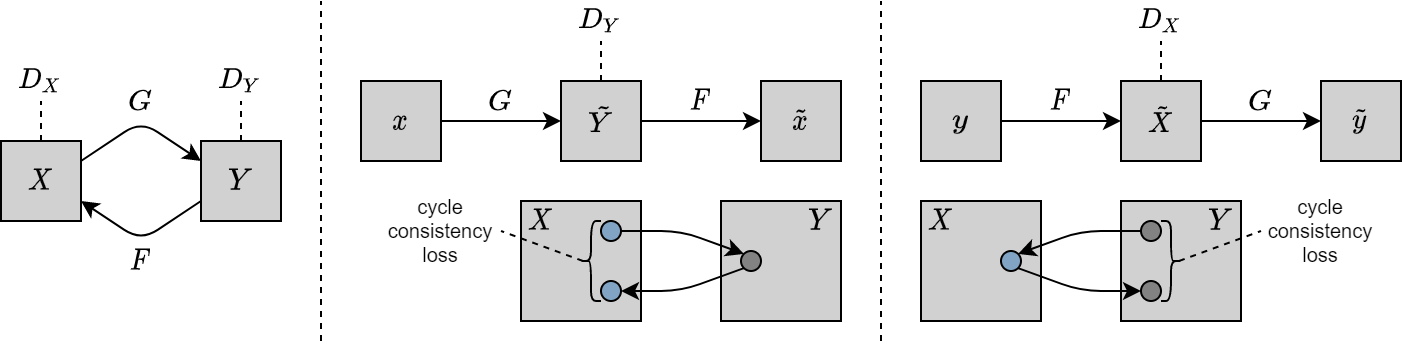
\includegraphics[width=\textwidth] {cyclegan_general_idea.png}
\centering
\caption{General idea of CycleGAN}
\label{fig:cyclegan_general_idea}
\end{figure}

CycleGAN networks have proven to be very efficient in many image-to-image translation problems. The most popular applications are:

\begin{itemize}
\item changing art styles in images of paintings
\item coloring black and white images
\item changing the season of the landscape in a photo
\item transforming horses into zebras
\item transforming apples into oranges
\end{itemize}